\documentclass[a4paper, 12pt] {article}

\usepackage[T1]{fontenc}
\usepackage{paralist}
\usepackage{amsmath}
\usepackage{romannum}
\usepackage{graphicx}

\graphicspath{{./images/}}
\newcommand{\head}[1]{\textnormal{\textbf{#1}}}

\begin{document}

\title{ECON-102: Principals of Microeconomics}
\author{Luka Trikha}
\maketitle

\begin{figure}[h]
    \centering
    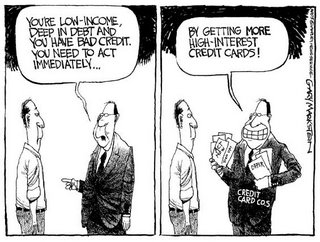
\includegraphics{cartoon.jpg}
\end{figure}

\newpage
\tableofcontents
\newpage

\section{Unit 1: Fundamental Concepts}
\subsection{Section 1: Economics}
In general terms, economics is defined as the study of how we can best increase
a nation's standard of living and citizens' happiness with the resources that we
have available to us.\\[2mm]
Standards of living include:
\begin{itemize}
    \item cars
    \item houses
    \item leisure time
    \item access to health care
    \item cleaner air
\end{itemize}

\subsubsection{Marginal Benefit \& Marginal Cost}
Marginal benefit and marginal cost can be though of as a positive cause-and-effect
in a business environment, with the benefit being the effect and cost being the
cause. When your marginal benefit is greater the marginal cost, the more likely
a positive investment is at play. For example, you may buy an expensive car for
your long commute, but it has the best MPG in the current car market and is 
heavily reliable (marginal benefit)--potentially outweighing the initial cost
(marginal cost).

\subsubsection{Difference between Macro- \& Micro- economics}
Macroeconomics focuses on the wider concepts that play a role on the entire
economy. Components of this include:
\begin{itemize}
    \item national unemployment rate
    \item inflation rate
    \item interest rate
    \item federal government budgets \& fiscal policies
    \item economic growth
    \item Federal Reserve System \& monetary policy
    \item foreign exchange rates
    \item balance of payments
\end{itemize}
Microeconomics deals with the smaller concepts of an economy such as:
\begin{itemize}
    \item supply and demand of individual goods and services
    \item price elasticity (sensitivity) of goods and services in demand
    \item production
    \item cost functions
    \item business behavior and profit maximization
    \item income inequality \& distribution
    \item effects of protectionism (tariffs, quotas, trade restrictions, etc.)
\end{itemize}
If macroeconomics is studying a forest, microeconomics is studying the
individual trees.

\subsection{Section 2: The Production Possibilities Curve}
\subsubsection{Production Choices}
Production choices are the idea that if you have limited resources to produces
various products, you want to optimize the resources at hand so that you can make
the most of the available resources, not under-use, and not over-promise a production
value that is not achievable.

\subsubsection{Points on the Curve and Trade-Offs}
In a given graph, any values that lie on the curve means that the operating cost
of the products are being used as efficiently as possible. The idea is that the
output cannot increase if it is limited by a constant resource and technology.
Scarcity talks about the limited resources at hand--which directly correlates
with the Production Possibility Curve. If a value lands on the curve, increasing
the production of one good/category will be at the expense of other goods/categories.
Points E, C, B, A, and D depicted in figure \ref{fig:GnR1} represents the most
optimized products that can be produced with resources at hand. It also shows
varying priorities for both Guns and Roses productions.

Any points that fall inside the curve (to the left of the curve, i.e point G in
figure \ref{fig:GnR1}) shows an inefficient use of resources to produce products.
Some reasons for this could be using fewer than the available resources
(unemployment), or using all resources but inefficiently (underemployment).

Points that fall outside the curve (to the right of the curve, i.e point G in
figure \ref{fig:GnR1}) shows a combination that cannot be achieved with the
available resources. This value does not mean point F will never be achievable--
the economy may grow and F may fall on or inside the Possibility curve, but at
the current analysis of the economy, it will not be possible.
Increases in technology and/or resources can help contribute to the growth of
the Production Probability Curve, which can help reach point F in the future.

\begin{figure}
    \centering
    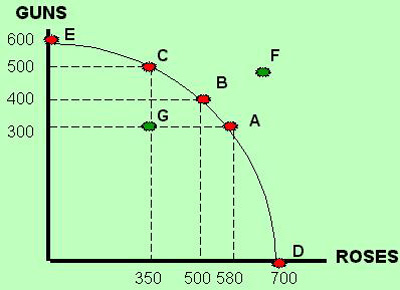
\includegraphics[width=7.5cm, height=5cm]{Production_Possibility_Curve.jpg}
    \caption{Example of a Possibility Curve of Guns and Roses production}
    \label{fig:GnR1}
\end{figure}

\subsection{Section 3: Economic Growth}
Economic growth occurs when the economy realizes greater production levels.
Essentially, when either the number of resources increase, or the way we use
resources becomes more efficient, is the only time the curve can shift outwards.
In short, economic growth is made possible by advances in technology and/or
increase in resources.

\begin{figure}
    \centering
    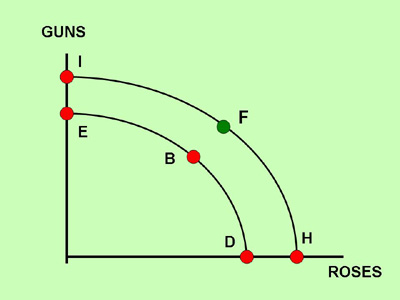
\includegraphics[width=7.5cm, height=5cm]{economic_growth_graph.jpg}
    \caption{Example of how economic growth now reaches point F}
    \label{fig:GnR2}
\end{figure}

\subsubsection{Increase in Capital Goods}
If a country is producing at full employment, more capital goods can be produced
only inf the country produces fewer consumption goods. A few ways governments
can encourage more production of capital goods can be through tax breaks for the
production of capital goods, or increasing taxes on the production/sale of
non-capital (consumption) goods.

\subsubsection{Advances in Technology}
Advancements in technology that contribute to economic growth are usually due to
entrepreneurs who have incentives to produce more efficiently and lower their
costs. When this model is successful, this usually drives the entrepreneur to 
continue to improve their models to become more efficient with both the work/effort
needed, and the money saved. Governments that allow entrepreneurs to keep most of
their profits and tax them less has been shown to produce greater rates of
technological growth. In addition to new technology, the more human technological
advancements made (greater education, training, skills, etc), the higher the 
production probability curve also grows.

\subsubsection{Economic Growth and Economic Systems}
There are various factors that can lead a country to economic growth and downfalls.
For example, in a capitalist country, having a government that supports just 
reward systems (taxes and regulations that reward work and entrepreneurship), 
just legal system, infrastructure, national security, and protection of individual
property rights can all lead to great economic growth. Also, political incentives
can also lead to economic growth. For example, India's switch to international 
trade in the 90's has led to greater opportunities, and the same for China in
the 80's when they adopted the free market elements.

Countries that practice communistic or command economy policies have seen 
significantly less economic growth due to the sheer control the government has
over resources and entrepreneurial entrepreneurial incentives.

In third world countries, instability with governments, corruption, civil strife,
national security, and uncertainty make is extremely difficult to have a 
steady, growing economy.

\subsubsection{Conditions for Economic Growth}
Countries with the highest per-capita earnings are characterized by all or most
of the following:

\begin{enumerate}
    \item \textbf{Strong private property rights.}

        If a country does not do its best to protect the property rights of its
        citizens, then the incentive to work hard in an economic state begins
        to dwindle. If a country allows the protection of private property to
        individuals, then incentive to work hard increases, since the properties
        (land, equipment, commodities, etc) is protected and belongs to the
        individual who earned it.

    \item \textbf{Free markets, free international trade, and a stable price level.}

        Free markets are markets in which prices of goods and services, wages, 
        rents, interest rates, and foreign exchange rates are determined by the
        interaction of private sector demand and supply.

        In order for free international trade, countries need to avoid protectionism
        (tariffs, quotas, etc.)

        Stable price level is achieved when there is little to no fluctuation
        in the country's average price level. This can be achieved by a country's
        monetary agency keeping its money supply restricted or constant.


    \item \textbf{Essential government regulations and reasonable levels of
        taxation.}

        Balanced rule, regulations, and taxes must be enforced by governments in
        order for governments to provide essential functions. If there is too 
        high of a tax, businesses and individuals will be less incentivized to
        work, while excessive regulations can lead to time consuming and 
        expensive business operations. If there are high taxes and excessive
        regulations, this discourages business start-ups, make businesses fail,
        or businesses may move abroad to avoid high taxes/regulations.

    \item \textbf{Little corruption.}

        If a governments/private groups initiates force by taking away citizen's
        businesses'/private property, it does not give any incentive for individuals
        to create/continue/maintain business with that government.
\end{enumerate}

The only cause of long-term economic growth and outward shifts in the production
possibility curve  are \emph{increases in resources and advances in technology}.
More and better resources allow businesses to produce more efficiently and 
effectively, lower costs, increase real incomes and increase purchasing consumers'
power. Increasing a nation's money supply or increased government spending 
\emph{may} help in the short-run, but has economic disadvantages in the long-run.
When wages are increased, that only means that the price of goods and services will
increase. There is no profit gain for businesses, and there is no money-saved
from consumers. The only thing that has changed is the \emph{nominal} prices of
wages, goods and services. The only way to increase real profits is to increase
productivity. This also lowers costs and decreases prices, which allows increases
in real profits and real demand.

\subsection{The Circular Flow}
The way how a basic economy works is that businesses offer goods, and households
pay businesses for those goods. Households also offer services to the businesses,
and in return, businesses pays the households for their services. Government also
plays a role, since they offer neutral services to both parties (households and
businesses). Since they offer services to both parties, the parties must also 
contribute to the government for those services (in the form of taxes).

When you bring in foreign markets into account, the same principals apply for
businesses, households, and governments.

Figure \ref{ref:circular_flow} is an illustration of the circular flow of a 
basic economy.
\begin{figure}[h]
    \centering
    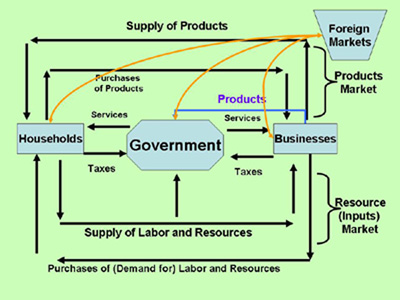
\includegraphics[width=7.5cm, height=5.0cm]{circular_flow.jpg}
    \caption{Graphical representation of how the circular flow works with 
    businesses, households, governments, and foreign markets.}
    \label{ref:circular_flow}
\end{figure}

\subsection{Economic Systems}
There are three different types of economic systems:
\begin{itemize}
    \item \textbf{Laissez-faire economy}
        represents a pure capitalist system (also called a price system). In this
        economy, the supply and demand behavior of businesses and households 
        determine the price of goods and services and factors of production. The
        government plays a very limited role and only provides the most essential
        functions such as a legal system, protecting individuals/property rights,
        and providing infrastructure and certain public goods.

    \item \textbf{Command economy}
        is a communist system where a country's government determines the prices
        of goods and services and factors of production. The country/government
        controls all of the country's economic decisions.

    \item \textbf{Mixed economy}
        is a mix between a command and laissez-faire economy. The exact mix of
        the two is dependent on the government involvement. Most industrialized
        countries follow this type of economic system.

\end{itemize}

\subsection{Important Concepts and Definitions}
Some definitions and concepts that will be used throughout these notes.

\subsubsection{Nominal and Real Values}
Nominal value (nominal wages, nominal interest rates, nominal Gross Domestic
Product, GDP) is the price of the actual dollar value which was recorded during
the transaction. This can be the price that shows up on a contract, receipt, etc.
You can think of this as the original monetary price of an invoice. Real value
is the monetary value that is reflective of the current market. For example,
lets say you bought a house 10 years ago for \$50,000, but its current market
value is \$100,000. The nominal value of the house is \$50,000, while the actual
value is \$100,000.

\subsubsection{Positive and Normative Economic Statements}
Positive economic statements are facts, or statements which can be proven. 
Positive statements does not have to be a true statement; the statement can be
proven false. It just needs to be provable. Examples of positive economic 
statements are:
\begin{itemize}
    \item The federal government experienced a budget surplus this past year
        (this is a false positive statement, but, by definition, a positive
        economic statement).

    \item When the value of the dollar falls, Japanese products imported into
        the United States become more expensive (this is a true positive statement).

    \item Legalizing drugs will reduce the drug profits that illegal drug dealers
        make (this is a true positive statement).

    \item The United States does not have a federally mandated minimum wage
        (this is a false positive statement).
\end{itemize}

A normative economic statement cannot be proven; they are opinions or value 
judgements. Examples of normative economic statements are:
\begin{itemize}
    \item The government should raise taxes and lower government spending to
        reduce the budget deficit.

    \item We need to try to lower the value of the dollar in order to discourage
        the imports of Japanese goods into this country.

    \item Our government should legalize the use of drugs in this country.

    \item The federal minimum wage should be at least \$15.00.
\end{itemize}

\subsubsection{Ceteris Paribus}
Latin for "if no other things in the economy change". When college tuition rises,
student enrollment will decrease, ceteris paribus. But if the parents' real income
increased as well, then student enrollment may increase, despite the tuition
increase. Therefore, the ceteris paribus condition is violated.

\subsubsection{Fallacy of Composition}
If you say what is good for one thing is \emph{necessarily} good for the entire
group, then you are subject to fallacy of composition. If a college has a
shortage of parking spots, your intuition is to tell students to arrive early.
But if every student comes early, there will still be a parking shortage issue.

\subsubsection{Broken Window Fallacy}
The idea that destruction stimulates the economy, therefore destruction creates
employment. This is not true. If you break a window, and hire a glazier to fix
it at the cost of \$500, the you have provided employment to the glazier. However,
if you did not break the window, you would have kept the \$500, and afterwards
you could buy a watch (which also increases employment). If you break the window,
you are gaining the employment of the glazier, but losing the employment of the
tailor. If you don't break the window, you will 1) keep the window, 2) keep the
\$500. 3) employ the tailor. Keeping the window is an important factor, since it
was already working, therefore there was no need to mindlessly destroy it in
order to hire a glazier. In general, destruction is not a good thing
microeconomicailly.

\subsubsection{Fallacy of Cause and Effect}
Basic idea of cause and effect; just because one action is immediately followed
by another action, does not mean action a caused action b to occur.

\subsection{Economics and Critical Thinking}
When looking at economic statements, scenarios, and analyses, you have to pay
attention and think about these six guidelines:
\begin{compactenum}
    \item \textbf{Question the source.}
        
        Study the background of the person making the statement to determine
        biases.
    \item \textbf{Question the assumptions.}

        Make sure you are not drawing conclusions too fast before thinking of 
        other factors that might come into play.
    \item \textbf{Question how the variables are defined.}
        
        The defining of variables is extremely important. If you are vague with
        the variables in your assumption, then you will have poor results, or
        the results you did not intend on happening. You can also be fooled by
        others' poor variable definitions, potentially swaying you and causing
        a sort of false-results. Garbage-in, garbage-out.
    \item \textbf{Question the validity of the statement.}

        Make sure the statements concluded do not fall into the fallacies, like
        the fallacy of cause and effect, and fallacy of composition (broken window
        fallacy).
    \item \textbf{Question the statistics.}

        Statistics can be meddled with, especially when you are vague with
        defining variables in your initial question.
    \item \textbf{Think like an economist.}
        
        Think practical in the sense of the real world and economics. Yes, maybe
        one solution passes the above five checks, but is it reasonable in the
        real world (outside of the math and conditions)?
\end{compactenum}



\end{document}
